%------------------ Präambel ---------------------------------------------------
\documentclass[envcountsame, envcountchap, deutsch]{i-studis}

\usepackage[utf8]{inputenc}

\usepackage[a4paper]{geometry}
\usepackage[english, ngerman]{babel}

\usepackage[pdftex]{graphicx}
\usepackage{epstopdf}

\usepackage{listings}

\usepackage[german, ruled, vlined]{algorithm2e}
\usepackage{amssymb, amsfonts, amstext, amsmath}
\usepackage{array}
\usepackage[skip=10pt]{caption}
\usepackage[usenames, dvipsnames]{color}
\usepackage[pdftex, plainpages=false]{hyperref}
\usepackage{textcomp}
\usepackage{hyperref}
\usepackage{csquotes}

%\usepackage{filecontents}

\usepackage{tikz}
\usepackage{pgfplots}
\pgfplotsset{compat=1.14}
\pgfkeys{/pgf/number format/.cd,1000 sep={\,}}

%\usepackage[numbers]{natbib} 
%\usepackage[english]{babel} 
%\usepackage[     %backend=biber,      natbib=true,     style=numeric,     sorting=none ]{biblatex}

%\begin{filecontents*}{eprint-hal.dbx}
%  	\ProvidesFile{eprint-hal.dbx}[2018/09/26 HAL/TEL eprints]
%	\DeclareDatamodelFields[type=field,datatype=verbatim]{arxiv,hal}
%	\DeclareDatamodelEntryfields{hal}
%	\DeclareDatamodelFields[type=field,datatype=literal]{arxivclass}
%	\DeclareDatamodelEntryfields{arxivclass}
%\end{filecontents*}
	
\usepackage[
    backend=biber,
    %backend=bibtex,
    style=numeric,%authoryear-icomp,
    sortlocale=de_DE,
    natbib=true,
    url=true, 
    doi=true,
	  datamodel=eprint-hal,
    eprint=true	
]{biblatex}

\usepackage{hyperref}

\DeclareFieldFormat{hal}{%
  \mkbibacro{HAL}\addcolon\space
  \ifhyperref
    {\href{https://hal.archives-ouvertes.fr/#1}{\nolinkurl{#1}}}
    {\nolinkurl{#1}}}

\DeclareFieldAlias{eprint:hal}{hal}
\DeclareFieldAlias{eprint:HAL}{eprint:hal}

\renewbibmacro*{eprint}{%
  \printfield{hal}%
  \newunit\newblock
  \iffieldundef{eprinttype}
    {\printfield{eprint}}
    {\printfield[eprint:\strfield{eprinttype}]{eprint}}}


\addbibresource{literatur.bib}

\usepackage{makeidx}
\usepackage{multicol}
\makeindex

\pagestyle{myheadings}
\setlength{\textheight}{1.1\textheight}

%\usepackage{showframe}
\lstset{
	basicstyle=\scriptsize\ttfamily,
	commentstyle=\scriptsize\ttfamily\color{Gray},
	identifierstyle=\scriptsize\ttfamily,
	keywordstyle=\scriptsize\ttfamily,
	stringstyle=\scriptsize\ttfamily,
	tabsize=4,
	numbers=left,
	numberstyle=\tiny,
	numberblanklines=false,
	frame=single,
	framesep=3mm,
	framexleftmargin=7mm,
	xleftmargin=10mm,
	linewidth=144mm,
	captionpos=b,
  xleftmargin=3mm, 
  xrightmargin=3mm,
}

%-- styles for code

\definecolor{codegreen}{rgb}{0,0.6,0}
\definecolor{codegray}{rgb}{0.5,0.5,0.5}
\definecolor{codepurple}{rgb}{0.58,0,0.82}
\definecolor{backcolour}{rgb}{0.95,0.95,0.92}

\lstdefinestyle{cpp}{
	  backgroundcolor=\color{backcolour},   
    commentstyle=\color{codegreen},
    keywordstyle=\color{magenta},
    numberstyle=\tiny\color{codegray},
    stringstyle=\color{codepurple},
    %basicstyle=\ttfamily\footnotesize,
    breakatwhitespace=false,         
    breaklines=true,                 
    keepspaces=true,                 
    numbers=left,       
    numbersep=5pt,                  
    showspaces=false,                
    showstringspaces=false,
    showtabs=false,                  
    tabsize=2,
}

%------------------ Manuelle Silbentrennung ------------------------------------
\hyphenation{Ele-men-tar-ob-jek-te ab-ge-tas-tet Aus-wer-tung House-holder-Matrix Least-Squares-Al-go-ri-th-men}


%------------------ Titelseite -------------------------------------------------
\begin{document}

\title{Implementierung eines Verfahrens zu effizienten Berechnung oszillierender Integrale}
\subtitle{Implementation of a method for the efficient calculation of oscillatory integrals}

\author{Tobias Arens}

\supervisor{Titel Vorname Nachname}

\address{Mehren}
\submitdate{08.10.2022}

%------------------ Projektart -------------------------------------------------
\project{Master-Abschlussarbeit}

\mytitlepage
\nocite{*}

%------------------ Vorwort, Kurzfassung, Verzeichnisse ------------------------
\frontmatter
\kurzfassung

%In der Kurzfassung soll in kurzer und prägnanter Weise der wesentliche Inhalt der Arbeit beschrieben werden. Dazu zählen vor allem eine kurze Aufgabenbeschreibung, der Lösungsansatz sowie die wesentlichen Ergebnisse der Arbeit. Ein häufiger Fehler für die Kurzfassung ist, dass lediglich die Aufgabenbeschreibung (d.h. das Problem) in Kurzform vorgelegt wird. Die Kurzfassung soll aber die gesamte Arbeit widerspiegeln. Deshalb sind vor allem die erzielten Ergebnisse darzustellen. Die Kurzfassung soll etwa eine halbe bis ganze DIN-A4-Seite umfassen.

%Hinweis: Schreiben Sie die Kurzfassung am Ende der Arbeit, denn eventuell ist Ihnen beim Schreiben erst vollends klar geworden, was das Wesentliche der Arbeit ist bzw. welche Schwerpunkte Sie bei der Arbeit gesetzt haben. Andernfalls laufen Sie Gefahr, dass die Kurzfassung nicht zum Rest der Arbeit passt.

In dieser Arbeit wird das in \citetitle{gasperini:hal-03209144} vorgestellte Verfahren implementiert. Basierend auf der Matlab-Implementierung der Autoren wurde eine hinsichtlich der Benutzbarkeit und Laufzeit eine verbesserte C++Implementierung umgesetzt.
Die Laufzeit der neuen Implementierung konnte im Vergleich nahezu halbiert werden und bei gleicher Genauigkeit der berechneten Integrale.  
Diese Verbesserungen wurden mithilfe von CPU-Parallelisierungen erreicht. 
Um die Implementierung einsetzen zu können werden ein Python-Modul sowie eine Matlab-Anbindung bereitgestellt.


\kurzfassungEN

In this paper, the method described in "An analysis of the steepest descent method to efficiently compute the 3D acoustic single-layer operator in the high-frequency regime".
is implemented. Based on the Matlab implementation of the
authors, an improved C++ implementation with respect to usability and runtime was implemented. The runtime of the new implementation has been
almost halved in comparison and with the same accuracy of the calculated
integrals. In order to be able to use this in a meaningful way, a Python module as well as a
a Matlab mex-file are provided.							% Kurzfassung/Abstract
\tableofcontents										% Inhaltsverzeichnis
\listoffigures											% Abbildungsverzeichnis (optional)
\listoftables											% Tabellenverzeichnis (optional)
\lstlistoflistings										% Listings (optional)


\lstset{
  inputpath=code,
  inputencoding = utf8,  % Input encoding
    extendedchars = true,  % Extended ASCII
    literate      =        % Support additional characters
      {á}{{\'a}}1  {é}{{\'e}}1  {í}{{\'i}}1 {ó}{{\'o}}1  {ú}{{\'u}}1
      {Á}{{\'A}}1  {É}{{\'E}}1  {Í}{{\'I}}1 {Ó}{{\'O}}1  {Ú}{{\'U}}1
      {à}{{\`a}}1  {è}{{\`e}}1  {ì}{{\`i}}1 {ò}{{\`o}}1  {ù}{{\`u}}1
      {À}{{\`A}}1  {È}{{\'E}}1  {Ì}{{\`I}}1 {Ò}{{\`O}}1  {Ù}{{\`U}}1
      {ä}{{\"a}}1  {ë}{{\"e}}1  {ï}{{\"i}}1 {ö}{{\"o}}1  {ü}{{\"u}}1
      {Ä}{{\"A}}1  {Ë}{{\"E}}1  {Ï}{{\"I}}1 {Ö}{{\"O}}1  {Ü}{{\"U}}1
      {â}{{\^a}}1  {ê}{{\^e}}1  {î}{{\^i}}1 {ô}{{\^o}}1  {û}{{\^u}}1
      {Â}{{\^A}}1  {Ê}{{\^E}}1  {Î}{{\^I}}1 {Ô}{{\^O}}1  {Û}{{\^U}}1
      {œ}{{\oe}}1  {Œ}{{\OE}}1  {æ}{{\ae}}1 {Æ}{{\AE}}1  {ß}{{\ss}}1
      {ç}{{\c c}}1 {Ç}{{\c C}}1 {ø}{{\o}}1  {Ø}{{\O}}1   {å}{{\r a}}1
      {Å}{{\r A}}1 {ã}{{\~a}}1  {õ}{{\~o}}1 {Ã}{{\~A}}1  {Õ}{{\~O}}1
      {ñ}{{\~n}}1  {Ñ}{{\~N}}1  {¿}{{?`}}1  {¡}{{!`}}1
      {°}{{\textdegree}}1 {º}{{\textordmasculine}}1 {ª}{{\textordfeminine}}1
      % ¿ and ¡ are not correctly displayed if inconsolata font is used
      % together with the lstlisting environment. Consider typing code in
      % external files and using \lstinputlisting to display them instead. 
}
%------------------ Kapitel ----------------------------------------------------
\mainmatter
\chapter{Einleitung und Problemstellung}

%Begonnen werden soll mit einer Einleitung zum Thema, also Hintergrund und Ziel erläutert werden.

%Weiterhin wird das vorliegende Problem diskutiert: Was ist zu lösen, warum ist es wichtig, dass man dieses Problem löst und welche Lösungsansätze gibt es bereits. Der Bezug auf vorhandene oder eben bisher fehlende Lösungen begründet auch die Intention und Bedeutung dieser Arbeit. Dies können allgemeine Gesichtspunkte sein: Man liefert einen Beitrag für ein generelles Problem oder man hat eine spezielle Systemumgebung oder ein spezielles Produkt (z.B. in einem Unternehmen), woraus sich dieses noch zu lösende Problem ergibt.
\section{Zielsetzung}

Basierend auf der Arbeit \citetitle{gasperini:hal-03209144}\cite{gasperini:hal-03209144} soll in dieser Arbeit das daraus resultierende Verfahren neu implementiert werden.
Die ursprüngliche Implementierung in Matlab funktioniert zwar, weißt aber Unzulänglichkeiten hinsichtlich der Benutzbarkeit und auch der Performanz auf.
So kann diese Lösung lediglich in Matlab verwendet werden und bietet keine Schnittstelle für Nutzer an. Des weiteren wurden keine Maßnahmen zur Optimierung der implementierten Lösung egriffen.

In dieser Arbeit sollen diese beiden Aspekte gelöst werden. Zum einen wird eine Implementierung angestrebt welche Paralellisierungstechniken verwendet um das Laufzeitverhalten zu verbessern, sowie eine API anbietet welche einfach verwendet werden kann.
Darüber hinaus soll die Benutzbarkeit mithilfe eines Matlab-Plugins und eines Python-Moduls erleichtert werden.
Wichtig dabei ist, dass die Implementierung keinen Verlust hinsichtlich der Genauigkeit der berechneten Integrale erleidet.



\section{Aufbau der Arbeit}

In Kapitel \ref{algo} dieser Arbeit wird zunächst das in \cite{gasperini:hal-03209144} entwickelte Verfahren vorgestellt und einige wesentliche Teilaspekte erläutert.
Danach werden in Kapitel \ref{desgin} die Entwurfsbedingungen erläutert und auf die konkreten Anforderungen sowie die geplante Architektur der Umsetzung eingegangen.
In \ref{plan} wird die Planung hinsichtlich der Optimierung erläutert, welche in Kapitel \ref{analysis} ausgewertet und präsentiert werden.
Im Kapitel \ref{impl} werden einige Details der Implementierung hervorgehoben, sowie die verwendeten Technologien vorgestellt.
\chapter{Das Verfahren}

In diesem Kapitel wird das zu implemnetierende VErfahren vorgestellt.
\section{Accoustic single-layer integral operator}

Welches Problem löst das Verfahren:
\begin{equation}
    \Delta
    I_{r,\Delta}(k) = \int_{\Delta}^{}  \frac{e^{ik(\left\lVert r-r'\right\rVert + \theta \cdot r')}}{\left\lVert r-r'\right\rVert} \,dr'
\end{equation}

Wie wird es im Paper angegangen:


\begin{equation} \label{eq:2}
    \Delta
    I_{r,\Delta}(k) = \int_{\Delta}^{}  \frac{e^{ik(\left\lVert r-r'\right\rVert + \theta \cdot r')}}{\left\lVert r-r'\right\rVert} \,dr'
\end{equation}

Und dann auf die relevanten Mathematischen "Grundlagen" eingehen die verwendet werden um das Verfahren implementieren:

\section{Mathematische Grundlagen}
\subsection{Cauchy-Integral-Theorem}




\subsection{Gauss-Laguerre Quadratur}

Die Gauss-Laguerre Quadratur ist eine Aproxmiation zur Auswertung von Integralen:
\begin{equation}
    \int_{0}^{\inf } f(t) e^-t  \,dt  \approx \sum_{i = 1}^{n} w_if(x_i) 
\end{equation}

Diese wird in dem steepest-descent Verfahren in Kombination mit dem Cauchy-Integral-Theorem genutzt um das Integral "LINK AUF FORMEL" zu berechnen.

\subsection{Steepest Descent Method}

In der Arbeit von \cite{gasperini:hal-03209144} wird das Integral \ref{eq:2} aus Formel 1 für ein Dreieck $\Delta \in \mathbb{R}^3$ und einen Einheitsvektor $\theta \in \mathbb{R}^3$ wie folgt definiert:
\begin{equation}
    I_{\Delta}(k) = | A_1 \times A_2 | \int_{0}^{1} \int_{0}^{1-y} \frac{e^{ik(\left\lVert Ax + b - r\right\rVert+\theta \cdot(Ax +b))}}{\left\lVert Ax + b - r\right\rVert }  \,dx \,dy 
\end{equation}
Dabei wird das Dreieck $\Delta$ als parametrisierties Einheitsdreieck mit der affinen Abbildung $x \mapsto Ax + $ mit $x = (x, y)^T, A \in \mathbb{R}^3$ und $b \in \mathbb{R}^3$ beschrieben.

Zusammen mit der Wellenzahl $k$ sind $A$, $b$, $r$ und $\theta$ die Eingabegrößen des zu implementierenden Algorithmus.
In Kapitel 2 von \cite*{gasperini:hal-03209144} wird hergeleitet wie die Gleichung \ref{2} in Abhängigkeit von diesen Eingabegrößen
definieren lässt.
Die Funktion $g$ in Gleichung \ref{2} lässt sich mithilfe der Funktion $P(x)$: 
\begin{equation}
    P(x) = c_0 x^2 + c_0|c|^2-2c_0xRe(c)
\end{equation}
wie folgt beschreiben:
\begin{equation}
    g(x) = \sqrt{P(x)} + qx + s
\end{equation}

 

\chapter{Entwurf}\label{desgin}
In diesem Kapitel wird auf verschiedene Aspekte der Entwurfsphase eingegangen.
Zum einen wird dargelegt, mit welcher Herangehensweise der Algorithmus umgesetzt wird und zum anderen werden die Entscheidungen über die verwendeten Technologien begründet.

\section{Anforderungen}

Ziel dieser Arbeit ist es, das in \cite*[]{gasperini:hal-03209144} beschriebene Verfahren zu implementieren.
Dabei sind drei Anforderungsbereiche auszumachen, welche in diesem Abschnitt behandelt werden.


\subsection{Korrektheit}

Die trivialste Anforderung ist, den beschriebenen Algorithmus korrekt zu implementieren.
Diese Anforderung ist erfüllt, wenn die Rechenresultate der Implementierung eine Genauigkeit der gleichen Größenordnung wie die MatLab-Implementierung von \cite*[]{gasperini:hal-03209144} erzielen.
Dort werden in Kapitel 6.1 (Tabelle 3) für die Parameter 
\begin{equation}
    A = \begin{pmatrix}
        0 & 0 \\
        2 & 0 \\
        0 & 2 \\
    \end{pmatrix}, b = \begin{pmatrix}
        0 \\ -1 \\ 0
    \end{pmatrix},
    r = \begin{pmatrix}
        0.6 \\ 0 \\0 
    \end{pmatrix},
    \theta = \begin{pmatrix}
        1 \\ 0 \\
    \end{pmatrix}
\end{equation}

die relativen Fehler des implementierten Verfahrens mit der Matlab \textit{integral}-Funktion für verschiedene Wellenzahlen $k$ verglichen.
\begin{table}[ht]
    \centering
    \begin{tabular}{|l|l|}
    \hline
    k & Relativer Fehler \\ 
    \hline \hline
    100  & $1.44 × 10^{-15}$ \\
    500  &  $1.15 × 10^{-14}$ \\
    1000 &  $9.71 × 10^{-5}$ \\
    3000 &  $5.11 × 10^{-7}$ \\
    5000 & $1.31 × 10^{-8}$ \\  \hline
    \end{tabular}    
    \caption{Genauigkeit der Implementierung von \cite*[]{gasperini:hal-03209144}}
\end{table} 
Das Kriterium der Korrektheit wird als erfüllt angesehen, wenn die Implementierung höchstens Fehler der gleichen Größenordnung liefert.


\subsection{Bedienbarkeit}

Die Anforderung der Bedienbarkeit wird im Rahmen dieser Arbeit wie folgt definiert:

\begin{enumerate}
    \item Es wird eine C++-Bibliothek bereitgstellt, welche mithilfe des Build-System \textit{CMake} eingebunden werden kann. 
    \item Es wird eine oder mehrere Matlab Mex-Funktionen ausgeliefert, welche den Algorithmus in Matlab benutzbar machen. 
    \item Es wird ein Python-Modul bereitgesellt, mit dem die 1D- und 2D-Algorithmen genutzt werden können.
\end{enumerate}

Dabei ist es nicht das Ziel, die beschriebenen Pakete offiziel auszuliefern. Das eigenhändige Compilieren der Bibliothek und gegebenfalls der Module ist erforderlich.

\subsection{Geschwindigkeit}\label{Performance}


Der implementierte Algorithmus darf nicht langsamer als die bereitgestellte Matlab-Implementierung sein.
Zu diesesm Zweck werden einige Auswertungen mit randomisierten Daten mithilfe von MatLab ausgeführt und direkt mit der vorhandenen MatLab-Implementierung verglichen.



\section{Architektur}

Diese Arbeit wird mit der Programmiersprache C++ umgesetzt.
Die Anwendung wird in drei Module aufgeteilt:
\begin{enumerate}
    \item Die Hauptbibliothek \texttt{steepest\_descent}, in welcher der eigentliche Algorithmus implementiert wird. Dort werden die \textit{Functor-Objekte} \texttt{integral\_1d} und \texttt{integral\_2d} bereitgestellt,
    welche den Python- und Matlab-Wrappern als Anknüpfpunkte dienen. 
    \item Das Python-Modul \texttt{stedepy}, welches diese Funktionalitäten inklusive einer Möglichkeit die für das Gauss-Laguerre benötigten Knoten und Gewichte zu berechnen.
    \item Das Matlab-Modul, welches sich aus mehreren Mex-Funktionen zusammensetzt, welche die Funkionen der API bereitstellen.
\end{enumerate}

\subsection{Klassendiagramm}

In Abbildung \ref{uml} wird ein vereinfachter Überblick über die implementierten Klassen und ihr Zusammenwirken gegeben.
Die Klassen \texttt{integral\_1d} und \texttt{integral\_2d} sind dabei die Schnittstellen für das Python- und das Matlab-Modul.
Die dargestellten Klassen sind verkürzt und die Funktionsparameter wurden ausgelassen, um die Lesbarkeit zu erhalten.

\begin{figure}
    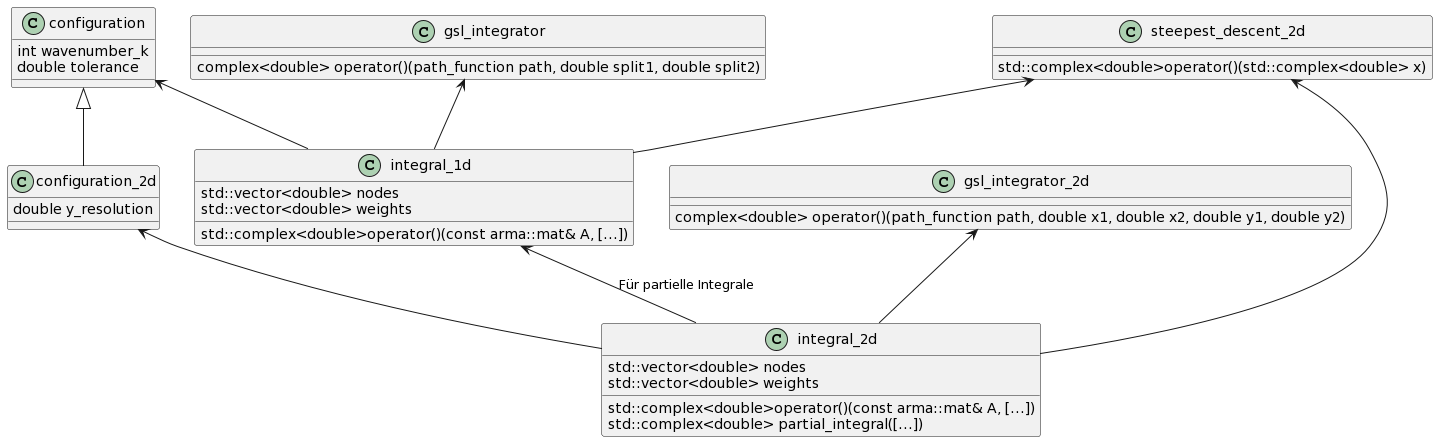
\includegraphics[width=\textwidth]{images/uml.png}
    \caption{Vereinfachtes UML-Diagramm der Implementierung}\label{uml}
\end{figure}

\pagebreak

\subsection{Parameter der Integration}

Die einzelnen API-Aufrufe teilen nur wenige gemeinsame Daten:
\begin{itemize}
    \item Die Wellenzahl $k$,
    \item den Beobachtungspunkt $r$,
    \item die Anzahl an Knoten für das Gauss-Laguerre-Verfahren,
    \item sowie die gewünschte Auflösung im zweidimensionalen Fall
\end{itemize}
Diese werden, abgesehen von dem Beobachtungspunkt $r$, in einer Konfigurationsklasse (siehe Abbildung \ref{configuration}) zusammengefasst.

\begin{figure}
    \lstinputlisting[language=C++,style=cpp]{configuration2d.cpp}
    \caption{Die Konfigurationen}\label{configuration}
\end{figure}


Die Parameter einer Integration eines Dreiecks teilen sich wie folgt auf:

\begin{itemize}
    \item Das Dreieck als parametrisiertes Einheitsdreieck, bestehend aus einer $2\times 3$-Matrix $A$ und einem Verschiebungsvektor $b$,
    \item der Beobachtungspunkt $r$,
    \item ein Richtungsvektor $\theta$
\end{itemize}

Zusätzlich wird noch der Beobachtungspunkt als Parameter mitgereicht, dies ermöglicht eine vollständige Kompabilität mit der Matlab-Implementierung.

\subsection{Functor-Objekte}\label{sec_functor}

Die Hauptkomponenten zur Integrationen werden als sogenannte \textit{Functor}-Objekte (Funktor) implementiert.
Diese Datenstruktur zeichnet sich dadurch aus, dass sie den C++-Funktionsaufrufsoperator bereitstellen und wie einfache C++-Funktionen aufgerufen werden können.
Da Funktoren durch Klassen bzw. \textit{structs} definiert werden, kann in ihnen ein Zustand gespeichert werden.
In Abbildung \ref{2d_integral_functor} ist die Header-Definition des Funktor für das Berechnen des zweidimensionalen Falls gezeigt.
In den Konstruktoren werden Parameter übergeben, welche für mehr als eine Integration invariant sind. In der Implementierung des Funktionsaufrufsoperators werden die im vorherigen Abschnitt definierten Parameter erwartet.

\begin{center}
    \lstinputlisting[language=C++,style=cpp]{2d_integral.hpp}
    \captionof{figure}{Funktordefinition der zweidimensionalen Integration}
    \label{2d_integral_functor}
\end{center}
\chapter{Vorgehensweise}


\begin{itemize}
    \item Einfache implementierung in simplen FUnktionen
    \item Hotpath-"Analyse"
    \item Parallelisierung mit OneTBB
    \item Evaluierung von Parallen Architekturen
\end{itemize}

Vorgehensweise zum Optimieren darlegen.

Historie der Implementierung ggf darstellen?

\section{Profiling}

Hotpath darstellen?


\section{Benchmarks}

Automatische Benchmarks mit Googlebenchmark => genereller Überblick

Implementiertes Matlab Plugin kann im direkten Verlgeich mit der origniallen Matlab Implementierung ausgeführt werden


\section{Manuelle Tests}

Manuelle TEsts + PRofiling haben gezeig,t dass in den TEsts der Hotpath wie erwartet der Fall ohne Singularität ist.
D.h. die Optimierung lohnt sich am meisten auf dem Hotpath! (Ambehls law oder wie hießt das?)

\section{Nicht berücksichtigte Optimierungen}

\begin{itemize}
    \item Verschiedene Compiler
    \item GPU beschleunigung: Numerische integrationsverfahren nicht auf GPU implementiert
\end{itemize}

\section{Architekturmodelle}


\chapter{Implementierung}

\section{Verwendete Technologien}


Mit Stern markierte gerne etwas weiter ausführen
\begin{itemize}
    \item Armadillo
    \item GNU Scientific Library *
    \item Pybind (Eigen3) *
    \item OneTBB *
    \item Catch2
    \item Google Benchmarks
    \item CMake
    \item Visualstudio Profiler
    \item Gprof (malsehen ob das noch genutzt wird)
    \item Valgrind*
\end{itemize}



Nicht genutzte Alternativen

Gründe noch aufführen
\begin{itemize}
    \item SIMD intrinsics * (mal sehen ob das sinnvoll ist)
    \item Boost numeric
    \item OpenCL
    \item OpenMP
    \item CUDA
\end{itemize}

\subsection{GNU Scientific Library}

Gerade bei der Frage nach dem Framework für Linalg und numerischer Integration lässt sich nicht abschätzen was die beste Lösung ist. Es gibt
so viele Frameworks und Bibliotheken, dass es nicht möglich ist alle gegeneinander Abzwuwägen.

Die Entshceidung GSL und Armadillo basier auf: Aramdillo ist einfach einzubinden und unkompliziert in der Anwendung.
GSL hat eine gute Perfomance. Der Verglecih lief mit Boost wobei einfache Tests zeigten das GSL schneller ist und mit weitaus weniger Aufwand in das Projekt integriert werden kann.
(Boost integration ist furchtbar!)


\subsection{Armadillo}

Kurze Einführng (1 Seite max?)

\subsection{Intel Threading Building Blocks}

Darstellung der beschleunigten Stellen, bzw beispiele wie man damit was parallelsiert + kurze einführenng

\subsection{Valgrind}

Erklärung der genutzten Tools Cachegrind und Cachetool?

\subsection{Pybind}

Kurze erklärung wie es klappt und beispiel für einfaches Plugin


\section{Ausgewählte Codestellen}

\subsection{Gauss laguerre integration und Cauchy Integral Theoerem}

\lstinputlisting[language=C++,style=cpp]{gauss_laguerre.cpp}

\subsection{1D Integration}



\subsection{2D Integration}

Warum konnte 1d Integration hier nicht direkt genutzt werden?
=> Indirektion durch das 1d Integral war relativ hoch, das teste ich aber besser noch mal
\chapter{Analyse und Auswertung}\label{analysis}


\section{Testsystem}

Die Performanztests wurden auf einem Vierkernprozessor Intel i5-4590 mit 8GB Arbeitsspeicher durchgeführt.


\section{Analyse mit Valgrind}

In diesem Abschnit wird auf die Analyse des Projektes mit Valgrind eingegangen. Zunächst werden Valgrind und die daraus benutzten Tools vorgestellt und dann werden einige Ergebnisse präsentiert.
\subsection{Valgrind}

Valgrind ist einerseits ein Framework zum Erzeugen von dynamsichen Analyse-Werkzeugen und andereseits eine Sammlung ebensolcher Werkzeuge (siehe \cite{10.1145/1250734.1250746}). 
Valgrind ist offene Software und wird unter der GNU GPL-2 Lizenz veröffentlicht\footnote{\url{https://valgrind.org/}}.
Die Sammlung bietet acht Werkzeuge\footnote{vgl. \url{https://valgrind.org/info/tools.html}} an von denen eines noch den Status eines experimentellen Werkzeugs hat:
\begin{itemize}
  \item Memcheck, ein Werkzeug zum Analysieren von Speicherlecks
  \item Cachegrind, ein Cache und Branch-prediction Profiler
  \item Callgrind, ein Profiler der einen Aufrufgraphen erzeugt
  \item Helgrind und DRD, Werkzeuge um Threading-Fehler zu erkennen
  \item Massif und DHAT, Heapprofiler für Analysen hinsichtlich speichereffizienter Programme 
  \item BBV, ein Werkzeug für die Forschung im Bereich der Rechnerarchitektur
\end{itemize}

In dieser Arbeit wurden die Werkzeuge Memcheck, Cachegrind und Callgrind verwendet. Die Ergebnisse der Werkzeuge DRD und Helgrind waren unbrauchbar, da diese nicht mit oneTBB kompatibel waren.

\subsubsection{Cachegrind und Callgrind}

Cachegrind und Callgrind, entwickelt von \citeauthor{Weidendorfer2004ATS} \cite{Weidendorfer2004ATS}, sind sogenannte Cacheprofiler. 
Diese Werkzeuge werden verwendet um die Programmstellen mit der größten Laufzeit festzustellen und verschiedene Umstellungen im Programmcode vergleichen zu können.

Cachegrind simuliert wie das zu testende Programm mit der Cache-Hierarchie und dem Branch-Predictor einer virtuellen Maschine interagiert. Die dabei simulierte Maschine ist orientiert an der Architektur moderner Maschinen.
Dabei werden verschiedene Caches simuliert und die Zugriffe darauf hinsichtlich von Misses ausgewertet. In Abbildung \ref{callgrind} ist ein Beispielaufruf zu sehen.
 

\begin{figure}
  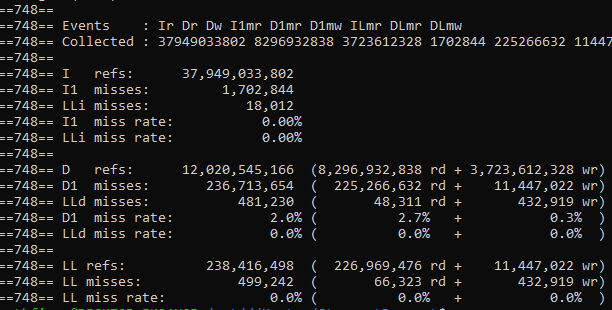
\includegraphics{images/callgrind.png}
  \caption{Beispielaufruf von Callgrind}\label{callgrind}
\end{figure}
%\subsubsection{Memcheck}

%Gehört eigentlihc nciht wirklcih hier her
%Screenshot plus was macht das Tool. Wir haben das genutzt um sicherzustellen, dass es keine Memoryleaks gibt.

\subsubsection{Auswerten von callgrind-Ergebnissen}


Mithilfe der Anwendung QCachegrind können die Ergebnisse von Valgrinds cachegrind/callgrind grafisch ausgewertet werden. QCachegrind ist ein Windowsbuild der Opensource Anwendung KCacheGrind.
KCachegrind ist Teil der Werkzeuge aus der Arbeit \cite{Weidendorfer2004ATS}.

\begin{figure}
  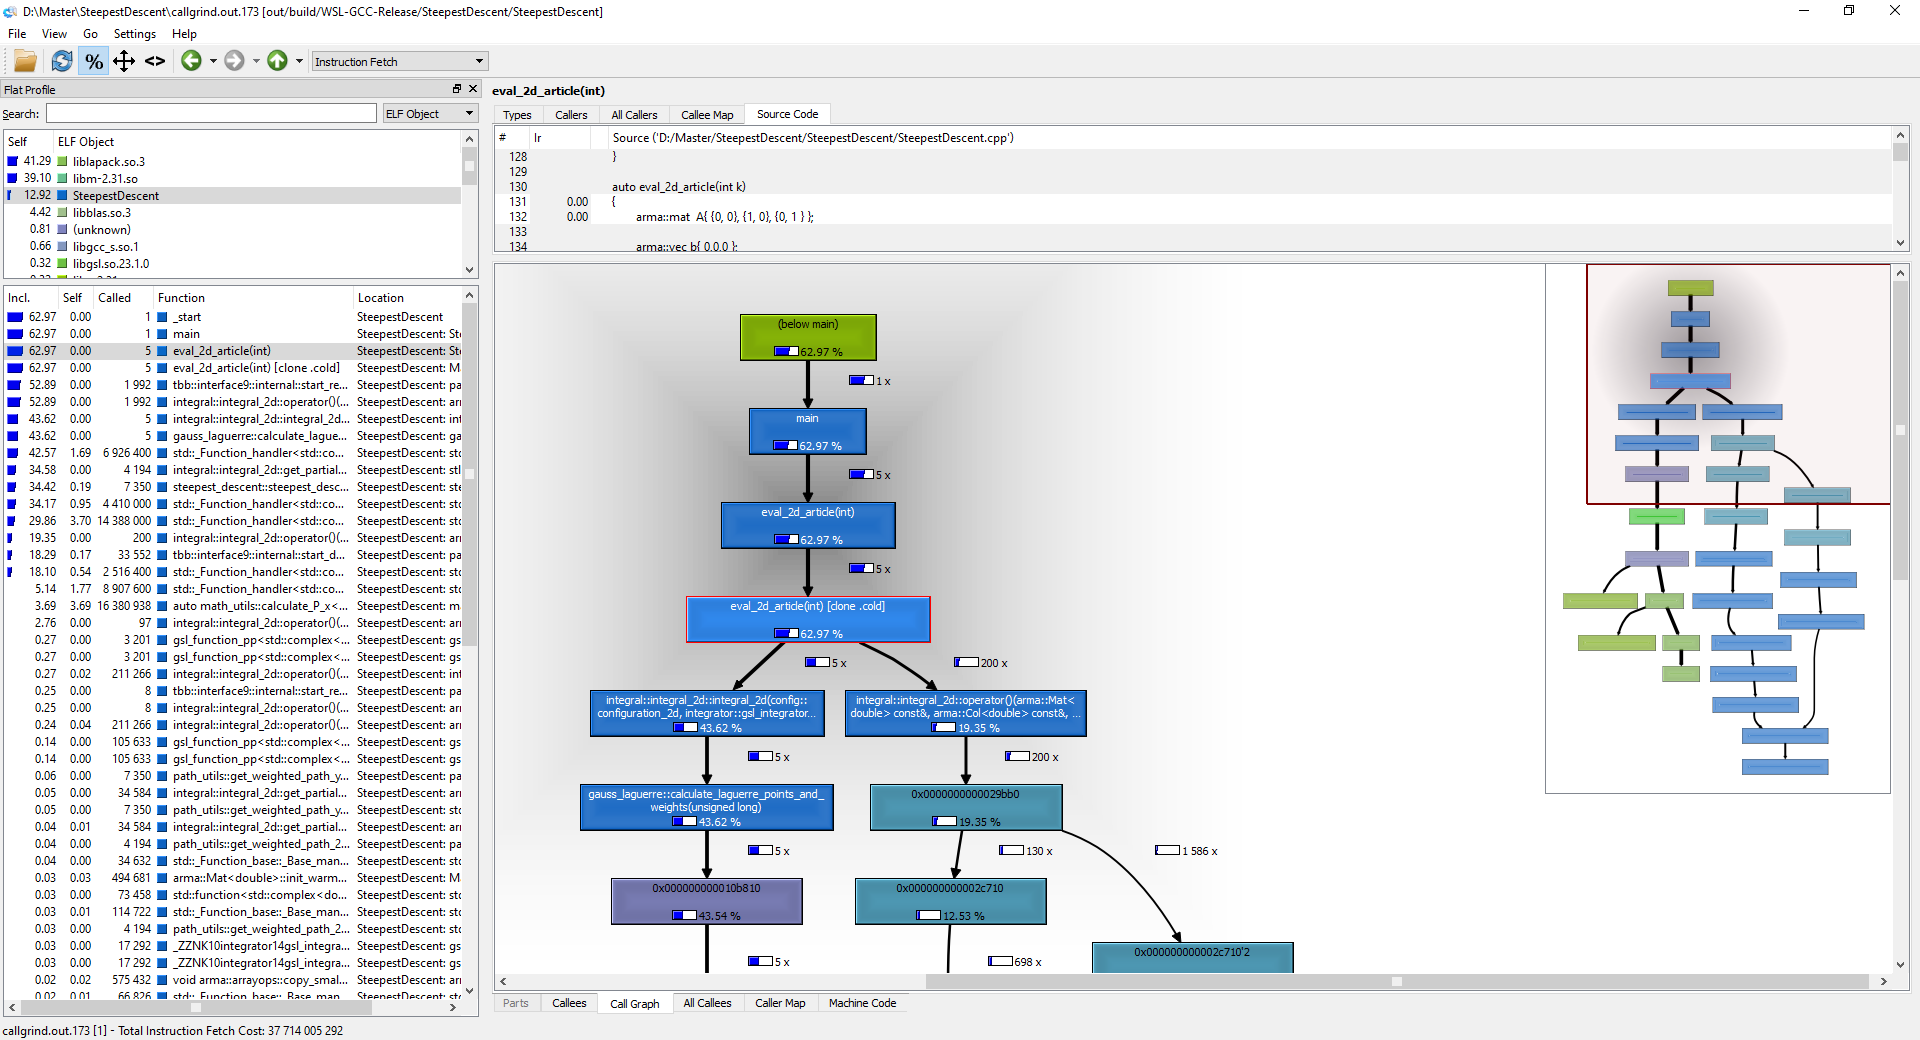
\includegraphics[width=\textwidth]{images/qcachegrind.png}
  \caption{Übersicht von QCachegrind}\label{qcachegrind}
\end{figure}

In Abbildung \ref{qcachegrind} ist eine Übersicht einer Auswertung mit QCachegrind zu sehen. In diesem Beispiel wurde mithilfe des Werkzeugs \texttt{callgrind} eine Aufzeichnung des zweidimensionalen Falls 
mit verschiedenen Wellenzahlen und jeweils 40 Stichproben von Beobachtungspunkt und Richtungsektoren für ein festes Dreieck berechnet.
Abbildung \ref{qcachegrind_result} stellt einen Ausschnitt des Aufrufgraphen vergrößert dar. In diesem lässt sich an Pfeilen ablesen wie oft welcher Programmteil aufgerufen wird und mithilfe einer prozentualen Angabe einsehen wie viel der Laufzeit in diesem Teil verbraucht wird.

\begin{figure}
  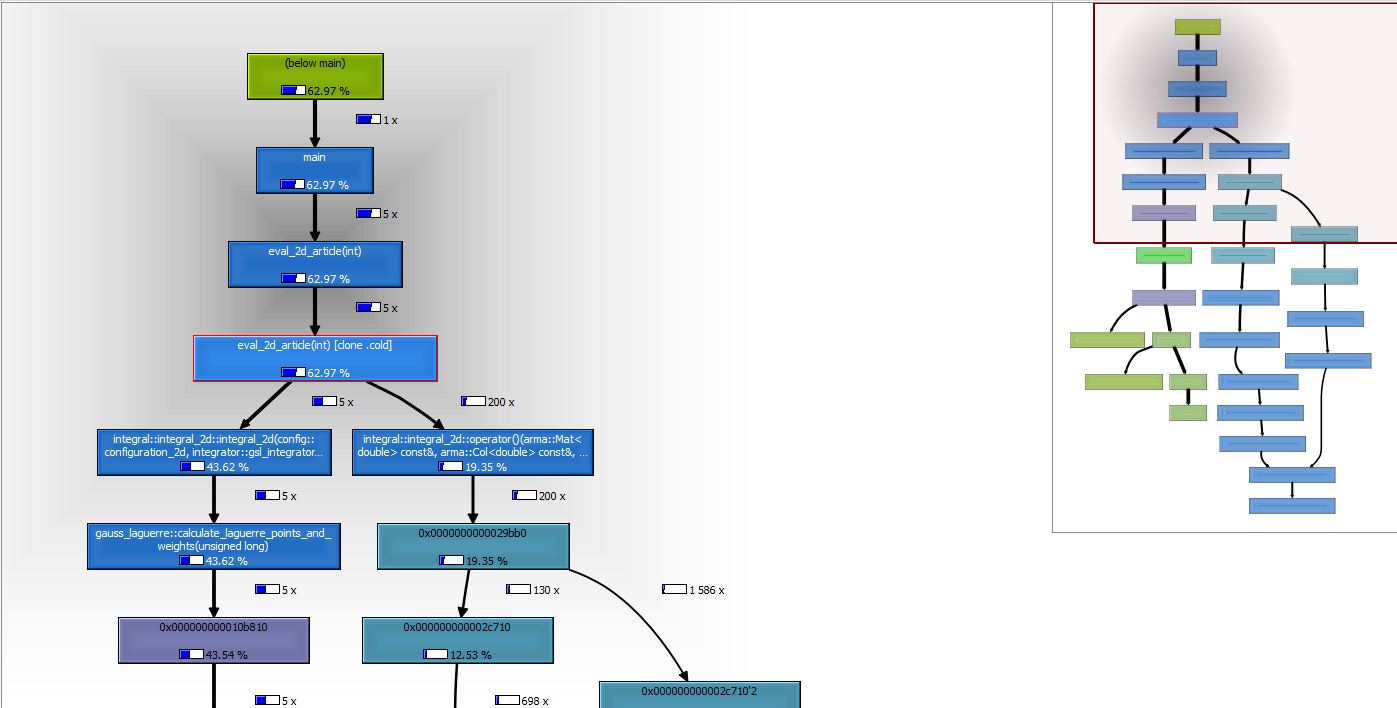
\includegraphics[width=\textwidth]{images/qcachegrind_callgraph.png}
  \caption{Aufrufgraph aus QCachegrind}\label{qcachegrind_result}
\end{figure}

Aus diesen und weiteren Auswertungen werden die meistaufgerufene Funktionen und der Hotpath ersichtlich.

\section{Ergebnisse der Optimierungsmaßnahmen}

In diesem Abschnitt wird auf einige Ergebnisse der manuellen Performanz-Messungen eingegangen.

\subsection{Hotpath}

Der häufigste Fall der Anwendung ist das Berechnen des Integrals in Situationen, in denen keine Singularität auftritt. 
Dementsprechend werden diese in den implementierten Funktionen als der Regelfall betrachtet.
Durch das vorziehen der Codestellen, die diese Szenarien abhandeln werden beispielsweise die benötigten Sprunganweisungen geringer gehalten.



\subsection{Meistaufgerufene Funktion}

Die Funktion mit der größten Laufzeit ist das \textit{Steepest-descent}-Verfahren.
Diese Funktion ist über mehrere Iterationen optimiert worden, bis sie die im Kapitel \ref{impl} dargestellte Form erreichte.
In früheren Versionen war dieses Verfahren in einer eigenen C++-Klasse implementiert, allerdings haben die Auswertungen gezeigt, dass ein
direkter Aufruf der Gauss-Laguerre-Quadratur einen Laufzeitgewinn von fast 50 Prozent erzielen lies.


\section{Auswertung der Laufzeitmessugen}

Die folgenen Laufzeitvergleiche wurden aus einer Matlab-Umgebung heraus ausgeführt, d.h. es werden die ursprüngliche Implementierung sowie das Matlab-Modul der C++-Implementierung verglichen.


\subsection{Iteration über Wellenzahl}


In diesem Test wird die Laufzeit hinsichtlich veränderter Wellenzahl \linebreak $k \in \{ 100, 500, 1000, 3000, 5000 \}$ gemessen.
Für jedes $k$ werden 50 zufällige Richtungsvektoren $r$ berechnet mit 600 Gauss-Laguerre-Knoten berechnet.

\begin{equation}
  A = \begin{pmatrix}
      0 & 0 \\
      1 & 0 \\
      0 & 1 \\
  \end{pmatrix}, b = \begin{pmatrix}
      0 \\ 0\\ 0
  \end{pmatrix},
\end{equation}

\begin{center}
    \begin{tikzpicture}
        \begin{axis}[
          width=\textwidth,
                  %width=3.358in,
        %height=2.309in,
        %at={(0.563in,0.312in)},
        scale only axis,
        yticklabel style={
          /pgf/number format/fixed,
          /pgf/number format/precision=2,
          /pgf/number format/fixed zerofill
        },
        extra y ticks={-0.05, 0.05},
        scaled y ticks=false,
        xlabel=Wellenzahl k,
        ylabel=\text{CPU-Laufzeit [s]},
        %xmin=0,
       % xmax=6000,
        %ymin=0,
        %ymax=0.5,
        axis background/.style={fill=white},
        legend style={legend cell align=left, align=left, draw=white!15!black}
        ]
        \addplot+[
      green, mark options={green, scale=0.75},
      smooth, 
      error bars/.cd, 
        y fixed,
        y dir=both, 
        y explicit ] table [color=green, mark=o, mark options={solid, green} x=k, y=t,y error=std, col sep=comma] { 
            k, t, std 
            100, 0.0546875000000000, 0.0377819439281490
            500, 0.0421875000000000, 0.0304832595619367
            1000, 0.0396875000000000, 0.0304767208961468
            3000, 0.0393750000000000, 0.0399597214296433
            5000, 0.0340625000000000, 0.0374428241844571         
          };
          \addplot+[
            red, mark options={red, scale=0.75},
            smooth, 
            error bars/.cd, 
              y fixed,
              y dir=both, 
              y explicit ] table [color=red, mark=o, mark options={solid, red} x=k, y=t,y error=std, col sep=comma] { 
                  k, t, std 
                  100, 0.120625000000000, 0.0825011595465820
                  500, 0.0928125000000000, 0.0439012055439740
                  1000, 0.0959375000000000, 0.0326549607327770
                  3000, 0.120625000000000, 0.164181352722021
                  5000, 0.0943750000000000, 0.0724645849462240          
                };
        %\addplot [color=red, draw=none, mark=o, mark options={solid, mycolor1}]
        %  table[row sep=crcr] file {..\data\performance_matlab.csv};
        \addlegendentry{C++ Implementierung}
        \addlegendentry{MatLab Implementierung}

        \end{axis}
    \end{tikzpicture}%
    \captionof{figure}{Laufzeitvergleich über verschiedene Wellenzahlen $k$, die Fehlerbalken zeigen die Standardabweichung}
\end{center}


\subsection{Laufzeitvergleich bei steigender Auflösung}


In diesem Test wird die Laufzeit hinsichtlich veränderter Auflösung $res \in \{ 0.1, 0.01, 0.001, 0.0001 \}$ gemessen.
Für jedes $k$ werden 50 zufällige Richtungsvektoren $r$ berechnet mit 600 Gauss-Laguerre-Knoten berechnet.

\begin{equation}
  A = \begin{pmatrix}
      0 & 0 \\
      1 & 0 \\
      0 & 1 \\
  \end{pmatrix}, b = \begin{pmatrix}
      0 \\ 0\\ 0
  \end{pmatrix},
\end{equation}
    
\begin{center}
    \begin{tikzpicture}
        \begin{axis}[
        %width=3.358in,
        %height=2.309in,
        %at={(0.563in,0.312in)},
        scale only axis,
        xmode=log,
        ymode=log,
        ymax=1000,
        width=\textwidth,
        %log ticks with fixed point,
        x dir=reverse,
        ylabel=\text{CPU-Laufzeit [s] (log)},
        xlabel=Layer-Auflösung (log),
        % for log axes, x filter operates on LOGS.
        % and log(x * 1000) = log(x) + log(1000):
        %x filter/.code=\pgfmathparse{#1 + 6.90775527898214},
        axis background/.style={fill=white},
        legend style={legend cell align=left, align=left, draw=white!15!black}
        ]
        \addplot+[
      green, mark options={green, scale=0.75},
      smooth, 
      error bars/.cd, 
        y fixed,
        y dir=both, 
        y explicit ] table [color=green, mark=o, mark options={solid, green} x=res, y=t,y error=std, col sep=comma] { 
            res, t, std
            0.1000,    0.0563,    0.0461
            0.0100,    0.3469,    0.0645
            0.0010,   3.8547,    1.6996
            0.0001,  38.9781,   15.6876
          };
          \addplot+[
            red, mark options={red, scale=0.75},
            smooth, 
            error bars/.cd, 
              y fixed,
              y dir=both, 
              y explicit ] table [color=red, mark=o, mark options={solid, red} x=res, y=t,y error=std, col sep=comma] { 
                  res, t, std
                  0.1000,    0.1375,    0.0799
                  0.0100,    0.8688,    0.0834
                  0.0010,    9.5406,    4.2787
                  0.0001,   86.2375,   27.7633
                };
        %\addplot [color=red, draw=none, mark=o, mark options={solid, mycolor1}]
        %  table[row sep=crcr] file {..\data\performance_matlab.csv};
        \addlegendentry{C++ Implementierung}
        \addlegendentry{MatLab Implementierung}
        \end{axis}
    \end{tikzpicture}%
    \captionof{figure}{Laufzeitvergleich über verschiedene Auflösungen, logarithmische Skalen, die Fehlerbalken zeigen die Standardabweichung}
\end{center}


\section{Vergleiche der Genauigkeit}

In diesem Abschnitt werden die numerischen Experimente aus Kapitel 6 von \cite{gasperini:hal-03209144} mit der in dieser Arbeit entwickelten C++-Implementierung durchgeführt.
Die Konfiguration ist wie folgt:

\begin{equation}
  A = \begin{pmatrix}
      0 & 0 \\
      2 & 0 \\
      0 & 2 \\
  \end{pmatrix}, b = \begin{pmatrix}
      0 \\ -0.5\\ 0
  \end{pmatrix},
  r = d \begin{pmatrix}
      cos(\alpha) \\ sin(\alpha) \\ 0
  \end{pmatrix} + \begin{pmatrix}
    0 \\ sin(\alpha) \\ 0
\end{pmatrix}, \theta \begin{pmatrix}
   1 \\ 0 \\ 0
\end{pmatrix}
\end{equation}\label{num_config}


\subsection{Eindimensionaler Fall}

Die Tests im eindimensionalen Fall werden wie in Kapitel 6.1 von \cite{gasperini:hal-03209144} mit 160 Gauss-Laguerre-Knoten durchgeführt.
Für die Konfiguration (siehe \ref{num_config}) und festgewählte $\alpha = 0$ und $d=0.6$ die relative Genauigkeit verglichen.
Diese Konfiguration enthält einen \textit{Splitting-point} in der Mitte des zu berechnenden Intervalls. (vgl Kapitel 6.1, Tabelle 3 in \cite{gasperini:hal-03209144})
In Tabelle \ref{accu} ist die Auswertung dieses Vergleichs zu sehen.

\begin{table}[ht]
  \centering
  \begin{tblr}{hlines,
      vlines,
      colspec={M{1.5cm}M{5cm}M{5cm}M{3cm}}}
      $k$ & C++-Implementierung & Matlab \textit{integral}-Funktion & Relativer Fehler \\
      100 &  $-0.07799217 + 0.13435696i$ &  $-0.07799217 + 0.13435696i$ & $1.12\times10^{-15}$ \\
      500 &   $0.04810768 + 0.05294844i$	&  $0.04810768 + 0.05294844i$ & $2.12\times10^{-14}$ \\
      1000 & $-0.03836233 + 0.03374236i$ &  $-0.03836224 + 0.03374733i$	& $9.71\times10^{-5}$ \\
      3000 & $-0.02377403 + 0.01807411i$	& $-0.02377404 + 0.01807412i$ & $5.11\times10^{-7}$ \\ 
      5000 & $-0.01930278 + 0.01243698i$	& $-0.01930278 + 0.01243698i$ & $1.31\times10^{-8}$ \\
  \end{tblr}
  \caption{Auswertung des Integrals $I(k,0,0,1)$ im Vergleich zu Matlab}\label{accu}
\end{table}

Im Vergleich des relativen Fehlers in diesem Versuch und Tabelle 3 aus \cite{gasperini:hal-03209144}
sind die relativen Fehler in ihrer Größenordnung gleichwertig. 
%In Tabelle \ref{accu_comp} wird der gleiche Versuch im Vergleich mit der 

%\begin{table}[ht]
%  \centering
%  \begin{tblr}{hlines,
%      vlines,
%      colspec={M{1.5cm}M{5cm}M{5cm}M{3cm}}}
%      $k$ & C++-Implementierung & Matlab \textit{Steepest-descent} & Relativer Fehler \\
%      100  & $-0.07799217 + 0.13435696i$ & $-0.07799217 + 0.13435696i$ & $1.44\times10^{-15}$ \\
%      500  & $ 0.04810768 + 0.05294844i$ & $ 0.04810768 + 0.05294844i$ & $1.06\times10^{-14}$ \\
%      1000 & $-0.03836233 + 0.03374236i$ & $-0.03836233 + 0.03374236i$ & $2.49\times10^{-15}$ \\
%      3000 & $-0.02377403 + 0.01807411i$ & $-0.02377403 + 0.01807411i$ & $1.04\times10^{-13}$ \\
%      5000 & $-0.01930278 + 0.01243698i$ & $-0.01930278 + 0.01243698i$ & $6.26\times10^{-14}$ \\    
%  \end{tblr}
%  \caption{Auswertung des Integrals $I(k,0,0,1)$ im Vergleich zur ursprünglichen Implementierung}\label{accu_comp}
%\end{table}



\subsection{Zweidimensionaler Fall}


Für den Test des zweidimensionalen Falls wird wieder auf festgewählte $\alpha = 0$ und $d=0.6$ zurückgegriffen.
Die Autoren schreiben in ihrer Auswertung, dass um die Berechnungen möglich sind mit geringeren Wellenzahlen $k$ getestet wird. (Siehe Kapitel 6.2 \cite{gasperini:hal-03209144})
Dies konnte in eigenen Tests nachvollzogen werden, da die Auswertungen von $k \in \{1000, 3000, 5000\}$ mehrere Stunden in Anspruch genommen haben.
Aufgrund eines Implementierungsfehler konnten diese Ergebnisse leider nicht verwertet werden, da dort die numerische Ungenauigkeit zu hoch war.

Zum  Vergleich wird die Funktion \textit{integral2} mit der Auflösung $res=0.0001$ über einzelne Schichten ausgewertet. Es wird die Wellenzahl $k=20$ verwendet.
Die Berechnung des Integrals mithilfe der Matlab Funktion wird in Abbildung \ref{matlab_integral} gezeigt. 
\begin{center}
  \begin{lstlisting}[language=MATLAB, breaklines]
    Im=0;
    count=0;
    for h = 0:res:1-res
          Im=Im+integral2(greenFun2D,0,1-count*res,count*res, (count+1)*res,'AbsTol',10^(-16),'RelTol',1e-8);
          count=count+1;      
    end
  \end{lstlisting}
  \captionof{figure}{Berechnung des 2D-Integrals in Matlab}\label{matlab_integral}
\end{center}

Die Ergebnisse dieses Vergleichs sind in Tabelle \ref{accu_2d} zu sehen.
\begin{table}[ht]
  \centering
  \begin{tblr}{hlines,
      vlines,
      colspec={M{1.5cm}M{5cm}M{5cm}M{3cm}}}
      $k$ & C++-Implementierung & Matlab \textit{integral2}-Funktion & Relativer Fehler \\
      5 & $-0.08447462 + 0.20608188i$ & $-0.0842793 + 0.20698190i$ & $4.1\times10^{-3}$ \\
      10 & $ 0.00682469 - 0.09068582i$ & $ 0.0066867 - 0.09105933i$ & $4.3\times10^{-3}$ \\
      20 & $ 0.02207955 - 0.02298169i$ & $ 0.0220181 - 0.02314369i$ & $5.4\times10^{-3}$ \\
  \end{tblr}
  \caption{Auswertung des Integrals $I_\Lambda(k)$ im Vergleich zu Matlab}\label{accu_2d}
\end{table}

%Im Vergleich zu der Auswertung in Tabelle 4 in \cite{gasperini:hal-03209144} fällt auf, dass die berechneten Integrale nicht übereinstimmen.

\chapter{Zusammenfassung und Ausblick}

In diesem Kapitel soll die Arbeit noch einmal kurz zusammengefasst werden. Insbesondere sollen die wesentlichen Ergebnisse Ihrer Arbeit herausgehoben werden. Erfahrungen, die z.B. Benutzer mit der Mensch-Maschine-Schnittstelle gemacht haben oder Ergebnisse von Leistungsmessungen sollen an dieser Stelle präsentiert werden. Sie können in diesem Kapitel auch die Ergebnisse oder das Arbeitsumfeld Ihrer Arbeit kritisch bewerten. Wünschenswerte Erweiterungen sollen als Hinweise auf weiterführende Arbeiten erwähnt werden.



%------------------ Literaturverzeichnis & Index -------------------------------
\backmatter
\printbibliography
%\bibliography{literatur}								% Literaturverzeichnis (literatur.bib)
\printindex												% Index (optional)


%------------------ Anhänge ----------------------------------------------------
%\begin{appendix}
%	\chapter{Glossar}

\abbreviation{DisASTer}		{Distributed Algorithms Simulation Terrain, eine Plattform zur Implementierung verteilter Algorithmen \cite{Gottwald:03}}

\abbreviation{DSM}			{Distributed Shared Memory}

\abbreviation{AC}			{Atomic Consistency (dt.: Linearisierbarkeit)}
\abbreviation{RC}			{Release Consistency (dt.: Freigabekonsistenz)}
\abbreviation{SC}			{Sequential Consistency (dt.: Sequentielle Konsistenz)}
\abbreviation{WC}			{Weak Consistency (dt.: Schwache Konsistenz)}
							% Glossar (optional)
%	\chapter{Selbstständigkeitserklärung}

\begin{description}

\item[$\Box$] Diese Arbeit habe ich selbstständig verfasst und keine anderen als die angegebenen Quellen und Hilfsmittel verwendet.\\

\item[$\Box$] Diese Arbeit wurde als Gruppenarbeit angefertigt. Meinen Anteil habe ich selbstständig verfasst und keine anderen als die angegebenen Quellen und Hilfsmittel verwendet.\\

Namen der Mitverfasser:
\vspace{3cm}

Meine eigene Leistung ist:
\vspace{3cm}

\end{description}

\vspace{3cm}

\begin{minipage}[t]{3cm}
	\rule{3cm}{0.5pt}
	Datum
\end{minipage}
\hfill
\begin{minipage}[t]{9cm}
	\rule{9cm}{0.5pt}
	Unterschrift der Kandidatin/des Kandidaten
\end{minipage}
	% Selbstständigkeitserklärung
%\end{appendix}


\end{document}
